\experiment{Dynamic Memory Allocation}{08/12/2023}

\section{Aim}
Implement boundary tag method of dynamic memory allocation using doubly linked list with FirstFit, BestFit and WorstFit allocation strategies. Also implement garbage collection and deallocation strategies.

\section{Algorithm}

 {\fontfamily{lmtt}\selectfont
  \subsection{Structures}
  \begin{enumerate}[label=\arabic*.,left=0pt]
    \item Define \texttt{block} structure with \texttt{size}, \texttt{isOccupied}, \texttt{next}, and \texttt{prev} attributes.
    \item Define \texttt{memory} structure with \texttt{totalSize}, \texttt{freeSize}, \texttt{head}, and \texttt{tail} attributes.
  \end{enumerate}

  \subsection{Function to Initialize Memory}
  \begin{enumerate}[label=\arabic*.,left=0pt]
    \item Create a function \texttt{initializeMemory(sizes, length)}:
          \begin{enumerate}[label=2.\arabic*.,left=0pt]
            \item Allocate memory for \texttt{memory} structure.
            \item Initialize \texttt{head} with the first block:
                  \begin{enumerate}[label=2.2.\arabic*.,left=0pt]
                    \item Allocate memory for the first \texttt{block}.
                    \item Set \texttt{size}, \texttt{isOccupied}, \texttt{next}, and \texttt{prev} attributes.
                    \item Set \texttt{head} and \texttt{tail} to the first block.
                  \end{enumerate}
            \item Initialize rest of the blocks:
                  \begin{enumerate}[label=2.3.\arabic*.,left=0pt]
                    \item Loop through the array \texttt{sizes} starting from index 1:
                          \begin{enumerate}[label=2.3.\arabic*.,left=0pt]
                            \item Allocate memory for a new \texttt{block}.
                            \item Set \texttt{size}, \texttt{isOccupied}, \texttt{next}, and \texttt{prev} attributes.
                            \item Link the new block to the previous block.
                            \item Update \texttt{tail} to the new block.
                            \item Update \texttt{totalSize} and \texttt{freeSize}.
                          \end{enumerate}
                  \end{enumerate}
            \item Return the created \texttt{memory} structure.
          \end{enumerate}
  \end{enumerate}

  \subsection{Function to Display Memory}
  \begin{enumerate}[label=\arabic*.,left=0pt]
    \item Create a function \texttt{displayMemory(m)}:
          \begin{enumerate}[label=2.\arabic*.,left=0pt]
            \item Print \texttt{totalSize} and \texttt{freeSize}.
            \item Loop through the blocks and print whether they are occupied or free.
            \item Loop through the blocks and print their sizes.
          \end{enumerate}
  \end{enumerate}

  \subsection{Function to Perform Garbage Collection}
  \begin{enumerate}[label=\arabic*.,left=0pt]
    \item Create a function \texttt{garbageCollect(m)}:
          \begin{enumerate}[label=2.\arabic*.,left=0pt]
            \item Loop through the blocks:
                  \begin{enumerate}[label=2.2.\arabic*.,left=0pt]
                    \item Check if the current block and its previous block are both unoccupied.
                    \item Merge the current block into the previous block.
                    \item Update \texttt{tail} to the previous block.
                    \item Free the current block.
                  \end{enumerate}
          \end{enumerate}
  \end{enumerate}

  \subsection{Function for First Fit Allocation}
  \begin{enumerate}[label=\arabic*.,left=0pt]
    \item Create a function \texttt{firstFit(m, size)}:
          \begin{enumerate}[label=2.\arabic*.,left=0pt]
            \item Loop through the blocks:
                  \begin{enumerate}[label=2.2.\arabic*.,left=0pt]
                    \item Check if the block is unoccupied and has enough size for the allocation.
                    \item Allocate the block for the required size.
                    \item If the block size is equal to the required size, return.
                    \item Create a new block for the remaining size and update the linked list.
                    \item If the allocated block is the last block, update \texttt{tail}.
                  \end{enumerate}
          \end{enumerate}
  \end{enumerate}

  \subsection{Function for Best Fit Allocation}
  \begin{enumerate}[label=\arabic*.,left=0pt]
    \item Create a function \texttt{bestFit(m, size)}:
          \begin{enumerate}[label=2.\arabic*.,left=0pt]
            \item Initialize \texttt{best} as \texttt{NULL}.
            \item Loop through the blocks:
                  \begin{enumerate}[label=2.2.\arabic*.,left=0pt]
                    \item Check if the block is unoccupied and has enough size for the allocation.
                    \item If \texttt{best} is \texttt{NULL} or the current block has a smaller size than \texttt{best}, update \texttt{best}.
                  \end{enumerate}
            \item If \texttt{best} is still \texttt{NULL}, print an error message and return.
            \item Allocate the block for the required size.
            \item If the block size is equal to the required size, return.
            \item Create a new block for the remaining size and update the linked list.
            \item If the allocated block is the last block, update \texttt{tail}.
          \end{enumerate}
  \end{enumerate}

  \subsection{Function for Worst Fit Allocation}
  \begin{enumerate}[label=\arabic*.,left=0pt]
    \item Create a function \texttt{worstFit(m, size)}:
          \begin{enumerate}[label=2.\arabic*.,left=0pt]
            \item Initialize \texttt{worst} as \texttt{NULL}.
            \item Loop through the blocks:
                  \begin{enumerate}[label=2.2.\arabic*.,left=0pt]
                    \item Check if the block is unoccupied and has enough size for the allocation.
                    \item If \texttt{worst} is \texttt{NULL} or the current block has a larger size than \texttt{worst}, update \texttt{worst}.
                  \end{enumerate}
            \item If \texttt{worst} is still \texttt{NULL}, print an error message and return.
            \item Allocate the block for the required size.
            \item If the block size is equal to the required size, return.
            \item Create a new block for the remaining size and update the linked list.
            \item If the allocated block is the last block, update \texttt{tail}.
          \end{enumerate}
  \end{enumerate}

  \subsection{Function for Freeing Memory}
  \begin{enumerate}[label=\arabic*.,left=0pt]
    \item Create a function \texttt{freeMemory(m, index)}:
          \begin{enumerate}[label=2.\arabic*.,left=0pt]
            \item Loop through the blocks:
                  \begin{enumerate}[label=2.2.\arabic*.,left=0pt]
                    \item Check if the block is occupied.
                    \item If the index matches the occupied block, free the block.
                    \item Update \texttt{freeSize}.
                    \item If the freed block is the last block, update \texttt{tail}.
                  \end{enumerate}
          \end{enumerate}
  \end{enumerate}

  \subsection{Main Function}
  \begin{enumerate}[label=\arabic*.,left=0pt]
    \item Initialize an array of block sizes.
    \item Initialize memory using \texttt{initializeMemory}.
    \item Display the initial state of memory using \texttt{displayMemory}.
    \item Allocate memory using worst fit, best fit, and free memory functions.
    \item Perform garbage collection.
    \item Display the final state of memory.
  \end{enumerate}
 }
\section{C Program}

\begin{lstlisting}[label={list:c_program2:graph-GraphAdjList}]
#include <stdio.h>
#include <stdlib.h>

typedef struct Block
{
  int size;
  int isOccupied;
  struct Block *next;
  struct Block *prev;
} block;

typedef struct Memory
{
  int totalSize;
  int freeSize;
  block *head;
  block *tail;
} memory;

memory *initializeMemory(int *sizes, int length);
void displayMemory(memory *m);
void garbageCollect(memory *m);
void firstFit(memory *m, int size);
void bestFit(memory *m, int size);
void worstFit(memory *m, int size);
void freeMemory(memory *m, int index);

int main()
{
  int sizes[10] = {1, 2, 3, 4, 5, 6, 8, 7, 9, 10};
  memory *m = initializeMemory(sizes, 10);
  displayMemory(m);
  worstFit(m, 7);
  displayMemory(m);
  bestFit(m, 6);
  displayMemory(m);
  bestFit(m, 5);
  displayMemory(m);
  garbageCollect(m);
  displayMemory(m);
  freeMemory(m, 0);
  displayMemory(m);
}

memory *initializeMemory(int *sizes, int length)
{
  memory *m = (memory *)malloc(sizeof(memory));
  // initialize first block
  block *head = (block *)malloc(sizeof(block));
  head->size = sizes[0];
  head->isOccupied = 0;
  head->next = NULL;
  head->prev = NULL;
  m->head = head;
  m->tail = head;
  m->totalSize = sizes[0];
  m->freeSize = sizes[0];
  block *prev = head;
  // initialize rest of the blocks
  for (int i = 1; i < length; i++)
  {
    block *new = (block *)malloc(sizeof(block));
    new->size = sizes[i];
    new->isOccupied = 0;
    new->next = NULL;
    new->prev = prev;
    prev->next = new;
    prev = new;
    m->tail = new;
    m->totalSize += sizes[i];
    m->freeSize += sizes[i];
  }
  return m;
}

void displayMemory(memory *m)
{
  printf("Total Size = %d, Free size = %d\n", m->totalSize, m->freeSize);
  block *current = m->head;
  int i = 0;
  while (current != NULL)
  {
    if (current->isOccupied)
    {
      printf("P-%d\t", i);
      i++;
    }
    else
    {
      printf("free\t");
    }
    current = current->next;
  }
  printf("\n");
  current = m->head;
  while (current != NULL)
  {
    printf("%dkb\t", current->size);
    current = current->next;
  }
  printf("\n");
}

void garbageCollect(memory *m)
{
  block *current = m->head;
  while (current != NULL)
  {
    block *next = current->next;
    m->tail = current;
    if (current->prev != NULL && !current->prev->isOccupied && !current->isOccupied)
    {
      current->prev->size += current->size;
      current->prev->next = current->next;
      if (current->next != NULL)
      {
        current->next->prev = current->prev;
      }
      m->tail = current->prev;
      free(current);
    }
    current = next;
  }
}

void firstFit(memory *m, int size)
{
  block *current = m->head;
  while (current != NULL)
  {
    if (!current->isOccupied && current->size >= size)
    {
      current->isOccupied = 1;
      m->freeSize -= size;
      if (current->size == size)
      {
        return;
      }
      block *new = (block *)malloc(sizeof(block));
      new->isOccupied = 0;
      new->size = current->size - size;
      new->prev = current;
      new->next = current->next;
      if (current->next != NULL)
      {
        current->next->prev = new;
      }
      current->size = size;
      current->next = new;
      if (current == m->tail)
      {
        m->tail = new;
      }
      return;
    }
    current = current->next;
  }
  printf("Required block is not currently avilable!\n");
}

void bestFit(memory *m, int size)
{
  block *current = m->head;
  block *best = NULL;
  while (current != NULL)
  {
    if (!current->isOccupied && current->size >= size)
    {
      if (best == NULL || best->size > current->size)
      {
        best = current;
      }
    }
    current = current->next;
  }
  if (best == NULL)
  {
    printf("Required block is not currently avilable!\n");
    return;
  }
  best->isOccupied = 1;
  m->freeSize -= size;
  if (best->size == size)
  {
    return;
  }
  block *new = (block *)malloc(sizeof(block));
  new->isOccupied = 0;
  new->size = best->size - size;
  new->prev = best;
  new->next = best->next;
  if (best->next != NULL)
  {
    best->next->prev = new;
  }
  best->size = size;
  best->next = new;
  if (best == m->tail)
  {
    m->tail = new;
  }
}

void worstFit(memory *m, int size)
{
  block *current = m->head;
  block *worst = NULL;
  while (current != NULL)
  {
    if (!current->isOccupied && current->size >= size)
    {
      if (worst == NULL || worst->size < current->size)
      {
        worst = current;
      }
    }
    current = current->next;
  }
  if (worst == NULL)
  {
    printf("Required block is not currently avilable!\n");
    return;
  }
  worst->isOccupied = 1;
  m->freeSize -= size;
  if (worst->size == size)
  {
    return;
  }
  block *new = (block *)malloc(sizeof(block));
  new->isOccupied = 0;
  new->size = worst->size - size;
  new->prev = worst;
  new->next = worst->next;
  if (worst->next != NULL)
  {
    worst->next->prev = new;
  }
  worst->size = size;
  worst->next = new;
  if (worst == m->tail)
  {
    m->tail = new;
  }
}

void freeMemory(memory *m, int index)
{
  block *current = m->head;
  int i = 0;
  while (current != NULL)
  {
    if (current->isOccupied)
    {
      if (i == index)
      {
        m->freeSize += current->size;
        current->isOccupied = 0;
        return;
      }
      i++;
    }
    current = current->next;
  }
  printf("Block with specified index not found!!");
}
\end{lstlisting}

\section{Output}
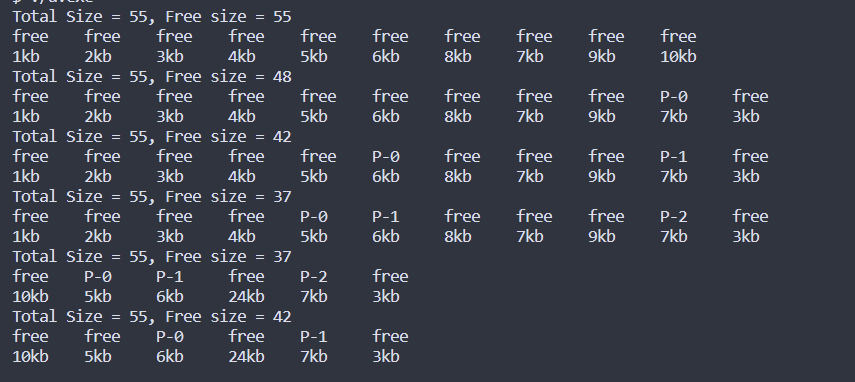
\includegraphics[width=\textwidth]{Cycle_2/Outputs/MemoryAlloc.png}

\section{Result}
Program is executed successfully, and output is verified.

